\chapter{Gradient learning}

Small math reminder $\nabla$ indicates derivatives: the derivatives on a function indicates the gradient (pendenza) on a point in the function so if positive we are growing in that point, if negative we are falling. Since we are using parable we only have 1 point with the derivatives = 0. 
\section{Gradient based learning}
Now we want to find the ERM on parametrized models, basically we want the minimum of the parametrized function. To achieve that we will use the gradient based method which consist in a iterative method that change based on what we obtain in the previous iteration.
What we have to do is construct a sequence of parameter vectors $w(0) \rightarrow w(1)$ that hopefully converge to a minimizer of f(w): $ f(\overline{w}) = \overline{f} := min f(w) $.

We approximate  locally $f(w)$ around $w^{(r)}$: $ f(w)\approx f(w^{(r)}) + (w-w^{(r)})^T \nabla f (w^{(r)})$ for w sufficiently close to $ w^{(r)}$.\\
Since we want to minimize f, we should go in the direction w such that $(w-w^{(r)})^T \nabla f (w^{(r)})$ is negative.\\
The next step has to be, given current guess w(r): $w^{(r +1)} = w^{(r)} - \alpha \nabla f(w^{(r)}) $ with a sufficiently small step size $\alpha >0$ and with $\alpha$ called learning rate.
\begin{figure}[H]
    \centering
    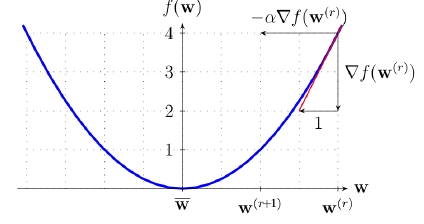
\includegraphics[scale=0.7]{images/GB/GB1.png}
    \caption{If $\nabla f(w^{(r)}) $ is positive, so in the right part of the minimum we have to go back in the left side with $- \alpha \nabla f(w^{(r)})$ called correction term, it will be the same if $\nabla f(w^{(r)}) $ was negative}
    \label{fig:enter-label}
\end{figure}

\subsection{Example: GD for linear regression}

We already know the ERM for linear regression that is $ \overline{w} = argmin f(w)$ with $  f(w) := \dfrac{1}{m} \sum\limits_{i=1}^m ( y^{(i)} - w^T x^{(i)})^2 $\\
If we compute gradient we obtain: $ \nabla f(w) = - \dfrac{2}{m} \sum\limits_{i=1}^m ( y^{(i)} - w^T x^{(i)}) x^{(i)} $\\
Then the gradient step is $ w^{(r)} := w^{(r-1)} + \alpha \dfrac{2}{m} \sum\limits_{i=1}^m ( y^{(i)} - w^T x^{(i)}) x^{(i)}$
\subsection{Choosing learning rate}
The problem now is,  how much is $\alpha$ need to be? It depends on the implementation and where we are because sometimes could be useful have big $\alpha$ to have a large step size and sometimes small step are recommended. In some cases, theoretical bounds and optimal values can be given but is \textbf{proved} that number of GD steps is smaller for standardized data. Another problem is when to stop, the solution can be have a fixed number of iteration (epochs) or when $ f(w^{(r-1)} ) - f(w^{(r)}) $ is less than a threshold or when validation error keep decreasing.

\section{Stochastic gradient descent}

The idea is to not use all the samples that could be billions, but use an approximation of the gradients descend :
\begin{itemize}
    \item Iteratively replace sum with a (random) component \\
    $g(w) := \nabla f_{i}(w) \quad w^{(r+1)} = w^{(r)} - \alpha \nabla f_{ir} (w^{(r)})$ 
    \item Iteratively replace sum with a (random) batch\\
    $ \mathbb{B} = \{ i_1, \dots , i_b\}  $ as batch $\quad g(w) = \dfrac{1}{\mathbb{B}} \sum\limits_{i' \in \mathbb{B}} \nabla f_{i'} (w)$
\end{itemize}

The idea is, instead of have less step on large samples is can be better have more step on fewer samples.

\section{Multi class classification}

Not all the classification can be binary but we want to have more label possible, often at the same time. There are different approach:
\begin{itemize}
    \item Naive approach: consider each label separately and solve problem separately for each label ignoring correlation (One vs rest trick)
    \item Multi class approach where each combination of label define a different categories, this means that the number of categories will be bigger
    \item Multi task learning approach: each individual label results in separate learning task and then combine the loss to learn together the two hypothesis
\end{itemize}

\section{Supervised learning techniques}
The supervised learning techniques can be divided into 2 different classes: the \textbf{regression} and the \textbf{classification}

\subsection{Regression}
\subsubsection{LASSO regressor}
LASSO (Least absolute shrinkage and selection operator) use regressor on a space of linear maps with datapoints with numerical features and label, the loss is the regularized squared loss.
Linear regression requires a training set larger than the number of features (m>n) to not overfit, but this is not a big issue considered that we can use regularization techniques with  penalty term in the loss for using too many features.\\
$L((x,y),h^{(w)} ) = (y -w^Tx)^2 + \lambda ||w||_{1} \rightarrow $ Increasing $\lambda$ results in a weight vector w with increasing number of zero coefficients and Works as a feature selection


\subsection{Classification}
\subsubsection{Support Vector Machines}

It is a classifier that can be extended as regressor and the datapoint must be numeric feature. The label values have to be binary; the model is a space of linear maps and the loss is the regularized hinge loss. The idea is to maximize the margin between different object in the hyperplane. The margin is the minimum distance of all closest point (missclassified have negative distance)
\begin{figure}[H]
    \centering
    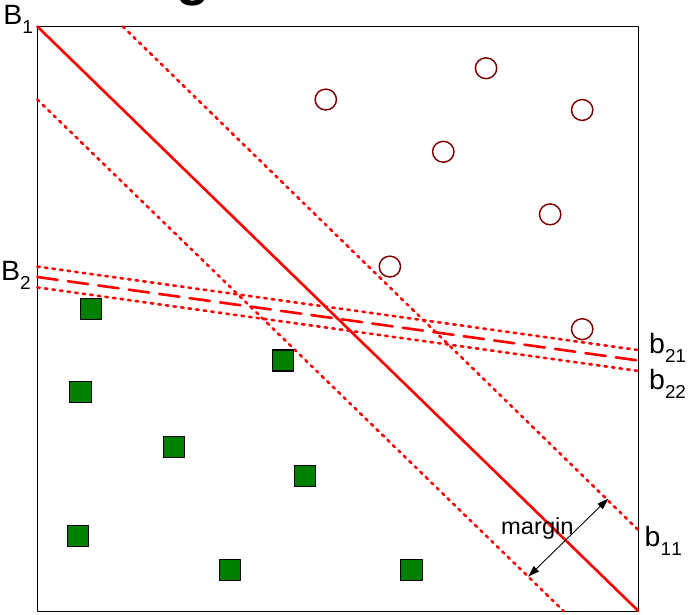
\includegraphics[scale=0.3]{images/GB/GB3.png}
    \caption{Caption}
    \label{fig:enter-label}
\end{figure}

The loss favors linear maps h(w) that are robust against (small) perturbations of the data points – more robust than logistic regressor

\subsubsection{Naive Bayes classifier}

Bayes classifiers are classifier that from a datapoint with numeric features give a 0/1 loss for every label using the Bayes rules ($ p(y|x) = \dfrac{p(x|y)* p(y)}{p(x)}$), the only problem is that We do not have this probability distribution $\rightarrow$ estimate it from training points because p(x) is constant for all y; p(y) is estimated by relative frequency of class y in the training set, but for p(x|y) we can only estimate

\begin{figure}[H]
    \centering
    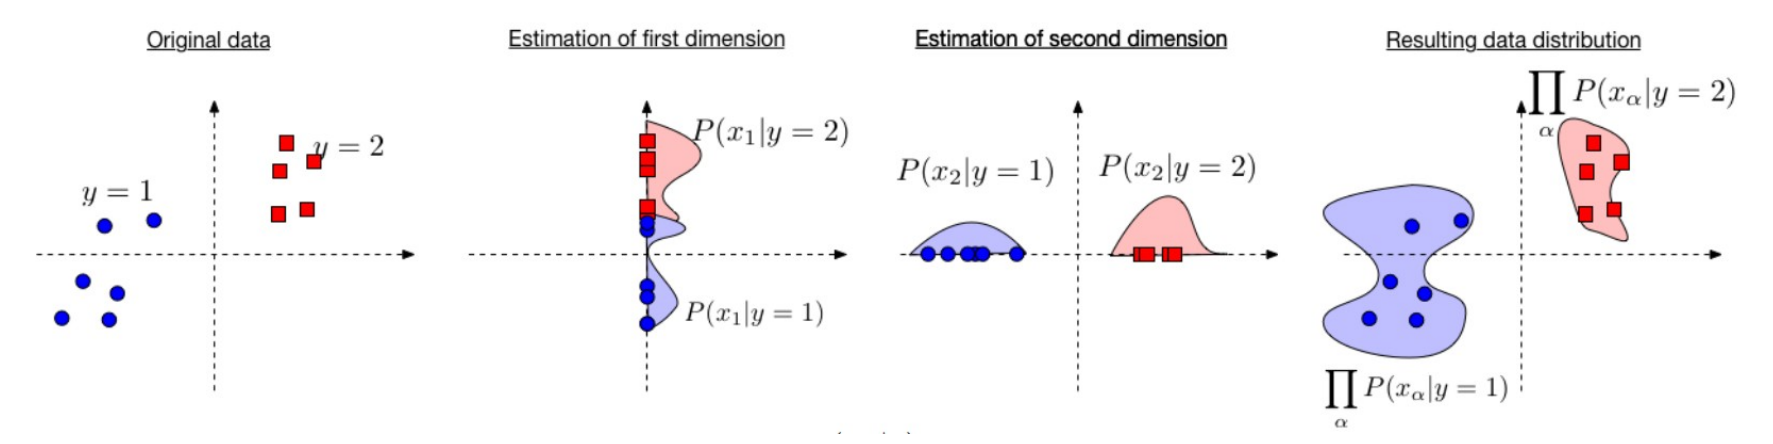
\includegraphics[scale=0.3]{images/GB/GB4.png}
    \caption{Caption}
    \label{fig:enter-label}
\end{figure}

$ h(x) = argmax_y p(y|x) = argmax_y \dfrac{p(x|y)* p(y)}{p(x)} $\\
$= argmax_y p(x|y)* p(y)$ because p(x) doesn't depend on y \\
$= argmax_y \prod\limits_{\alpha=1}^d p(x_{\alpha}|y)* p(y)$ by the naive Bayes assumption\\
$= argmax_y \sum\limits_{\alpha=1}^d log(p(x_{\alpha}|y)) * log(p(y))$ as log is a monotonic function

It is important to know that Naive Bayes is a linear classifier and a variant called Gaussian Naive Bayes where we assume x as a Gaussian with mean and variance depending on y
\subsubsection{Decision Tree and Random Forest}
Decision tree are models that uses a tree-like model of decisions and their possible outcomes/classes and contains only conditional control statements. There are many algorithms like Hunt's, CART, ID3 C4.0, C5.0. Are useful because allows non-linear regression and are very fast and easy to interpret.  In regression, the trees output a single number per leaf node instead of a label.

Random forest  is an ensemble classifier that consists of many decision trees, For each tree of the K trees of the forest, choose a subset of n’ features (n is the total number of features) and a subset of m’ training data (m is the total number of samples)
 \begin{figure}[H]
     \centering
     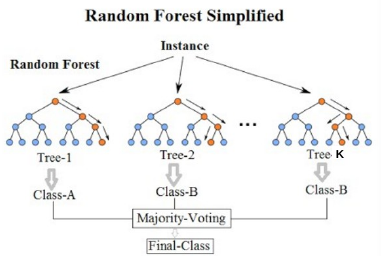
\includegraphics[scale=0.8]{images/GB/GB6.png}
     \caption{Caption}
     \label{fig:enter-label}
 \end{figure}
 There is also a visualizer for them.
\subsubsection{K-nearest neighbors}
 Uses k closest points for performing classification/regression, the choice of the k is important because too big or too small can cause problem.
 \begin{figure}[H]
     \centering
     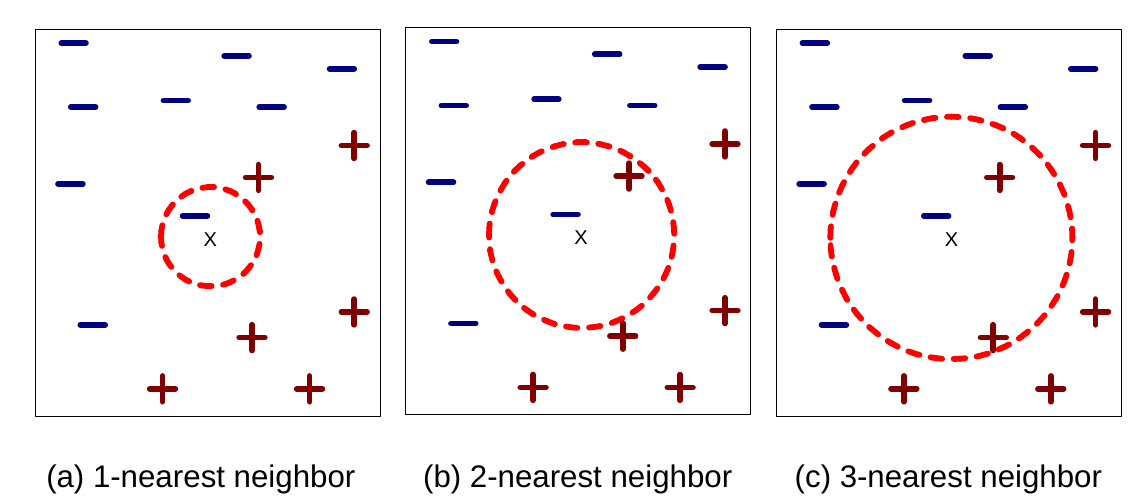
\includegraphics[scale=0.5]{images/GB/GB5.png}
     \caption{Caption}
     \label{fig:enter-label}
 \end{figure}